% arara: pdflatex: {files: [mainfile]}
% !arara: indent: {overwrite: true}
{\itshape This document describes the life of (Edward) Michael Hughes (Grandad). It was
	originally written with great affection by his eldest grandson, Chris, based on a few discussions in late 2013; after
	his death, further additions were made by the rest of Grandad's family, most notably by his son, Richard. Most folks that read this
	document would probably have known Grandad as `Mike' or `Michael'. We all remember him very fondly, and will
	miss him dearly; we hope that this memoir will help to highlight some of his many achievements, and the
various chapters of his life.}

\paragraph{March 21st 1925} Grandad was born in Balham, London.
\paragraph{1928} Grandad moved out to Ash Road in Morden with his parents where his Dad was working on the telephone exchange;
Grandad remembers the advert said, 'Come and live in rural Surrey'; the lifestyle and commute was facilitated
by the tube which had been extended from inner London and enabled a whole
wave of people to move out to Surrey. Grandad remembers being asked by
his mother, `Do you like it here, Michael?', to which he responded, `Yes, let's go home now'.

Grandad lived here in Ash road with his parents from 1927--1959, apart from the four years he served
in the RAF from 1943-1947.  The area was built up over a long period of time;
the house was surrounded by fields---Grandad named the fields: `the chicken's field',
`the rabbit's field', `the builder's field', but he said that they all became `builder's'
fields eventually. At the end of the garden there
was an orchard which was the last bit to be developed. On one occasion Grandad went under the
fence with his Dad to pick apples for his Mum to make jam---the old lady that owned the field
found them out and waved her walking stick and yelled, 'trespassers', and his
Dad said, 'Come on Michael, let's run for it'.

\paragraph{1930} Grandad met Ron, who would be his life-long best friend, at primary
school---the teacher asked Grandad to sit next to Ronny Lewis. Grandad and Ron were key members
of a gang that shared many similarities with the outlaws from `Just William', by Richal Compton.

\paragraph{1933} Grandad was a boy scout around this time; he progressed to patrol leader of the Peanut
patrol, and recalled reciting, `Dib, dib, dib, dob, dob, dob'.

\paragraph{1942} Grandad volunteered for the RAF at the age of seventeen and a half, but
was rejected as he did not have his father's written permission.
\paragraph{1943-1947} Now aged eighteen, and not needing permission, Grandad reapplied to the RAF.
There was no national service---soldiers were simply called up for the `the present
emergency'.
\begin{wrapfigure}{R}{5cm}
	\centering
	\rotatebox{-90}{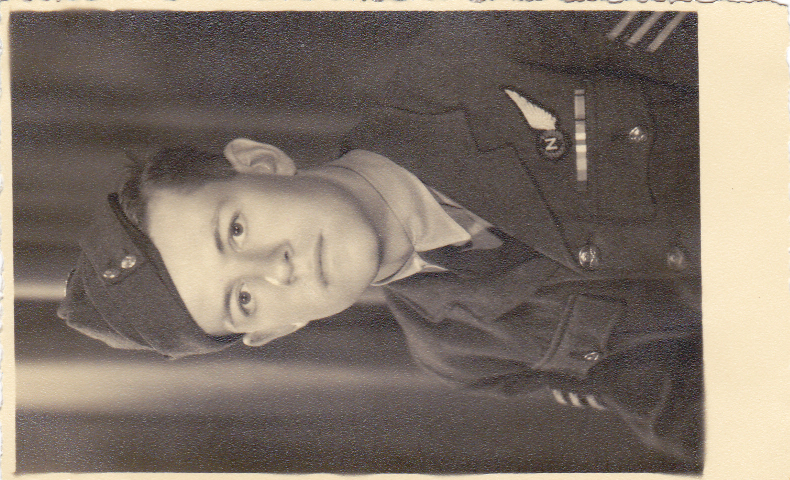
\includegraphics[width=.7\textwidth]{portrait}}
\end{wrapfigure}
Grandad reported to the recruit center in central London (near Lord's cricket ground);
marched up the road to a nice block of flats opposite Regent's Park with London Zoo.
All the furniture had gone, and there were only beds.
The drill corporal regularly compared the recruits with the monkeys on the other side of the canal.
After three weeks of exercises (such as marching up the road, standing at ease), they were transferred to a training
center in Newquay (Cornwall) which coincided with the middle of the summer; it was
one of the best summers England had seen in years. As long as they (the recruits) reported to duty when they needed to,
they could go in the sea whenever they liked.

They would do physical training on the beach, ending with an hour's swimming in the (very rough) sea.
On one occasion Grandad and a friend of his decided that they would run along the beach to explore---they found a
cove. The rising water trapped them on the cliff,  so they spent the night on the side of the cliff, which the
weather allowed as it was a nice summer.  As they returned to the camp they saw that the squadron was lined up outside;
it turned out that the entire squadron was looking for them. Grandad and his friend
were charged with irresponsible behaviour and marched before the commanding officer, still
only with their bathing trunks. The commanding officer wanted to avoid the paper work, so just
gave them a reprimand and told them to 'piss off'.

The recruits were shipped out from Newquay to Manchester (in a grounds that was a public park during peace
time), then to Liverpool Lyme-street station on a train where they marched through the town onto a ship,
and onto South Africa.  As they marched through Liverpool girls would open their windows from the offices and
cheer them on, sometimes crudely.

The ship sailed via the Atlantic ocean and the Gilbralta Straights as part of a convoy with one cruiser and many corvettes to Durban (South Africa).
There was a a horrendous storm where the stern of the ship came out of the water (including the propeller);
the ships were rocking so hard that some of the ships were on their side.

They slept in hammocks on board ship; a lot of the soldiers
didn't like sleeping in hammocks, so the folks that did like it had quite a lot room. Grandad describes this as
one of the more pleasant experiences---the hammock would lessen the amount of rocking from the
sea, so by and large he didn't feel sick. The food on the troop ship was quite good compared
to what the folks at home were getting---the bread was baked fresh every day but the flour was
infested with weevils, so they would have to go through it and pick them out.

\begin{wrapfigure}{R}{5cm}
	\centering
	\rotatebox{-90}{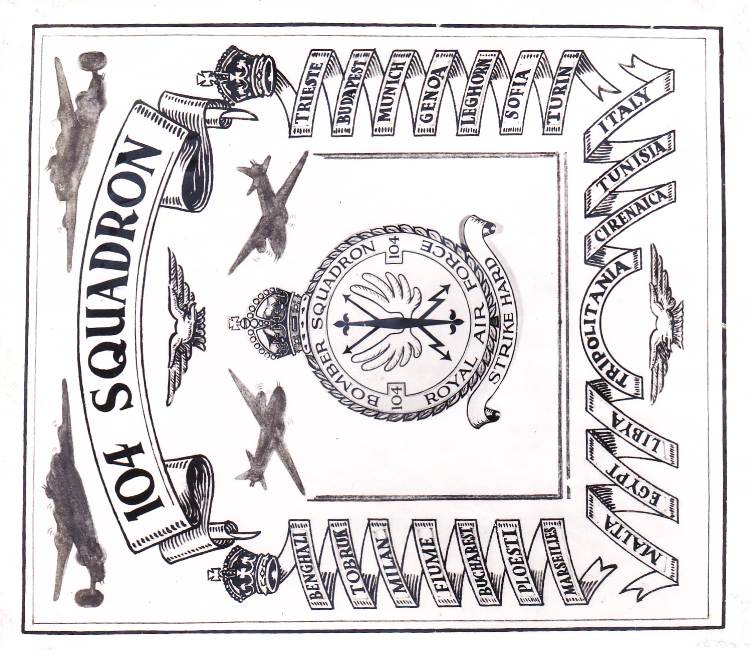
\includegraphics[width=.6\textwidth]{squadron104}}
\end{wrapfigure}
On one occasion in South Africa, Grandad went to the cinema; at the end of the film
the (British) National anthem was played (as was the tradition at this time), and several of the
locals protested their disapproval by putting their hats on and sitting down.

\paragraph{Squadron 104} The recruits were flown up to Egypt on a flying boat to complete the training, and
then travelled by troop ship to Foggia, a poverty-stricken part of southern Italy.

Grandad joined Squadron $104$ in February 1945; at this time it was well known that
the war was close to finishing, which meant that some folks felt some relief. The
squadron stayed in tents on the edge of a field; the Sergeant's mess was set up
in a farm house where the soldiers would get food, and there were couches to rest upon.
The previous occupants of the farm house were forced to live with their livestock.

\paragraph{Missions} Grandad's squadron flew in the four-engined, American-made Liberator air craft (not to be
confused with the Lancaster bomber). They
took supplies (mainly underwear and warm clothing, not guns and ammunition, which surprised Grandad)
and materials to Serbia. Their drop site would
be marked in a field with a big white `X', and they would fly over at about 1000ft, and push
the parachute-prepared crates out. They often watched people emerge from the woods with carts,
who would then collect the supplies, and disperse.
The night-time missions were to bomb railway stations in various small towns in Serbia and northern Italy (Verona),
as the Germans were using them to bring in supplies. One place outside Verona had a movable bridge---the
intelligence had not reported that the bridge could move, which resulted in 104 squadron dropping bombs into
the river.

\paragraph{1947} The English government
decided to integrate returning veterans slowly into society to prevent the labour market being
flooded, so when the war had finished the squadron was moved to Egypt (Grandad preferred the Italians, though).
During this time, a
representative from the civil service spoke to the soldiers about opportunities once their
service had finished. Grandad took the exam, and was offered the job. Each soldier was given
a number, and told to wait until their number came up.
\begin{wrapfigure}{R}{5cm}
	\centering
	\rotatebox{-90}{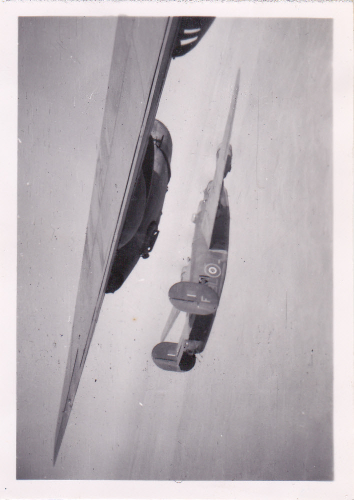
\includegraphics[width=.25\textwidth]{liberator}}
\end{wrapfigure}

Grandad and Ron arranged to meet during his time in Egypt. Ron had a job
in air transport, and was responsible for organizing planes travelling from England
to the middle East. Grandad arranged a fortnight's leave, as did Ron, who
managed to arrange free transport to Cairo (Grandad had to pay for his from
the Canal zone). They stayed in the `Woes and Joes', a Bed and Breakfast where RAF memebers
could stay without fear of being assaulted. They took a bus out to the pyramids, a place
that was (and is still) popular with tourists.

Grandad and Ron met Eric Schofield, whom they knew from their school days. They
took him out for some drinking, and felt duty bound to bring him back to his tent (he was
at a transit camp in the desert). They shoved him into his tent, assuming that
the floor would be soft; they were duly surprised when Eric arrived the next day
covered in bruises---it transpired that the tents had concrete floors. After this,
Grandad and Ron stayed in a posh hotel in Alexandria, where they were given
a list of safe places to stay. They spent their time swimming in the sea
and sitting in the sunshine.

On Grandad's 21st birthday he remembers delibrately \emph{not} telling anyone, as
he wished to avoid the tradition of having to buy everyone a drink.

Grandad finished his tour and had six weeks leave, so went back to live with his parents, which was
very common at the time---young men typically lived with their parents until they married.

\paragraph{1947} One of Grandad's fondest memories is coming home from the RAF in 1947; his Dad knew
he was coming home  as the country had relaxed from the tension of the war.
One could phone a number and ask for the status of a ship. Grandad arrived home at
11 o clock at night; his Dad said, `Hello Son' as if he'd only been away for
a couple of days (even though he had been away for four years); he heard a noise
behind him and it was his Mum coming down the stairs to greet him.

Grandad worked at a station controlling fighter aircraft in Essex, in a stately manner at a table
with holes and strings; he would take calls from lost pilots, triangulate their position
and help them go in the correct direction.

During this period, Grandad's `number' came up, and he travelled to Blackpool for
civil service training. On the way \emph{to} the training, the soldiers were loaded from
the train into a lorry, and had to clamber over the sides to enter it. On the
way back \emph{from} the training, they were treated like civilians, and were
given a set of steps to exit and enter the vehicle---they had been `de-mobbed' (de-mobilized).

\paragraph{1947--1952} Grandad tried to get Ron elected as an MP to the Labour party. \fixthis{expand on this!}

\paragraph{1952} Grandad met Granny Hat, joined the revenue and worked in an office
in the west end of London; the building has since been demolished, and in its stead
stands the new Scotland Yard.
Grandad used to have work-hosted Christmas parties at an old pub called, `The Feathers', which still stands by its side.
It was at one such party that Grandad introduced Granny Hat to his colleagues---one woman
assumed that she was his sister.

\paragraph{1956} Grandad moved into his first house in Beulah Road with Granny Hat and their son, Richard.
\paragraph{1967} The family moved to 34 East Drive, which followed from Grandad's promotion within
the Inland Revenue Service.
\paragraph{1969} Grandad's Dad had good health up until the few weeks before he died; one
of the things that Grandad felt guilty about for quite a time was leaving him on his own. Granny Hat  wanted
a place to raise a family in her own place.
\paragraph{1988} Grandad and Granny Hat Moved to Southbourne to be closer to the family. Grandad
has lived in Southbourne longer than anywhere else since he was de-mobbed.

\paragraph{August 28th, 2014} Grandad died peacefully in his sleep in his favourite chair at 4 South Lane, Southbourne; he will be missed by all of those
who knew and loved him, and remembered dearly as a man who approached life with a wonderful attitude
towards life.

\begin{tikzpicture}[
		man/.style={minimum height=.75cm,rectangle,draw,fill=blue!20},
		woman/.style={minimum height=.75cm,rectangle,draw,fill=red!20,rounded corners=.8ex},
		grandchild/.style={grow=down,xshift=1em,anchor=west,
			edge from parent path={(\tikzparentnode.south) |- (\tikzchildnode.west)}},
		level 1/.style={sibling distance=15em},
		level 2/.style={sibling distance=-5em},
		level 3/.style={sibling distance=6em},
         first/.style={level distance=6ex},
           second/.style={level distance=12ex},
             third/.style={level distance=18ex},
		%level 1/.style={sibling distance=10em}]
	]
	% Parents
	\coordinate
	child[grow=left] {node[man,anchor=east]{Gabriel Edward Hughes}}
	child[grow=right] {node[woman,anchor=west]{Sally Constance Cuming}}
	child[grow=down,level distance=0ex]
	[edge from parent fork down]
	child{
		node[man] {(Edward) Michael}
		child[grow=right,xshift=2cm]{node[woman] {Pat Jewitt}}
		child {
			node[man]{Richard}
			child[grow=right,xshift=1cm] {node[woman]{Theresa Lyons}}
			child[grandchild,first] {
                node[man]{Chris}
			    child[grow=right,xshift=.5cm] {node[woman]{Marisa Moon}}
                }
			child[grandchild,second] {node[man]{David}}
			child[grandchild,third]{node[woman]{Katie}}
		}
	}
	child {node[woman]{Pamela}
		child[grow=right,xshift=1cm]{node[man] {Keith Beard}}
		child {node[man]{Anthony}}
		child[xshift=4cm] {node[woman]{Hilary}}};
\end{tikzpicture}
\end{document}
